\chapter{LLMを用いた話しことば検出 \label{c7}}

本章では,LLMを用いた話しことばを検出させる実験について述べる.LLMが持つ話しことばの知識を本システムの話しことばルールを比較し,ChatGPTがもつ話しことばの認識について調査した。

\begin{comment}
書きことばリストは、話しことばチェッカーで検出しない表現をもとに選んでいる。
それでもchatGPTが出力する場合は、チェッカーの癖もあり得る。← これは要相談
\end{comment}
\section{7.1 \label{c7s1}}
本実験で用いたデータは,本学で2019年度に開講された「アルゴリズムとプログラミング」の講義内で提出されたレポートの16件を取り出し,それらのレポートの本文である.

\subsection{検証方法}
プロンプトの構成は,ChatGPTに役割を与える「役割」,取り組んでほしいタスクを示した「指示」,「話しことばの具体例」,「書きことばリスト」,「学生のレポート本文(検出をさせる文章)」の5段構成である.

\begin{table}[H]
\centering
\caption{話しことば検出のためのプロンプト(前半部)}
\small % \footnotesize
\begin{tabular}{|l|}
\hline
\multicolumn{1}{|c|}{プロンプト} \\ \hline
\begin{tabular}[c]{@{}l@{}} 
\#\#\# 役割 \#\#\# \\
あなた(GPT)を,「大学初年次における日本語文章教育のエキスパート」と\\します。\\
\\
\#\#\# 指示 \#\#\# \\
以下の<話しことば具体例>を参考に、\#\#\# 学生のレポート課題の文章 \#\#\#の\\
文章から話しことばにあたる単語をすべて検出してください。\\
出力は\#\#\# フォーマット \#\#\#に従ってください。
なお、公的文書や学術論文、技術文書などで\\使用されるフォーマルな表現を書きことばとします。\\
敬語や丁寧語の文章や日常生活で出てくる文章で使用される表現を話しことばとします。\\
話しことばの具体例は、以下の<話しことば具体例>に載せています。\\
ただし、以下の<書きことばリスト>は話しことばではないので、検出しないでください。\\
<話しことば具体例>\\
1. (~して)いて\\
2. うまく\\
3. かもしれない\\
4. こういった\\
5. (~もある)し\\
6. (~)して\\
7. そんな\\
8. たくさん\\
9. たら\\
10. ていて\\
11. てしまう\\
12. とても\\
13. どんな\\
14. なので\\
15. ので\\
16. (文末の)ます。\\
17. わからない\\
18. 思う\\
19. 私\\
20. 色々\\
21. 素晴らしい\\
22. 分からない\\
\end{tabular}   \\ \hline
\end{tabular}
\label{prompt-detectspoken-api}
\end{table}
\begin{table}[H]
\centering
\caption{話しことば検出のためのプロンプト(後半部)}
\small % \footnotesize
\begin{tabular}{|l|}
\hline
\multicolumn{1}{|c|}{プロンプト} \\ \hline
\begin{tabular}[c]{@{}l@{}} 
<書きことばリスト>\\
1. 考える\\
2. 考えられる\\
3. 使う\\
4. 使われている\\
5. だろう\\
6. ている\\
7. このように\\
8. である\\
9. わかる\\
10. だろうか\\
11. できる\\
12. できるだろうか\\
13. のではないだろうか\\
14. ではないだろうか\\
15. ためである\\
16. つまり\\
17. そもそも\\
18. このような\\
19. どのような\\
20. この\\
21. その\\
22. あの\\
23. どの\\
24. 様々な\\
25. ならば\\
26. 使っている\\
27. この場合\\
28. 学ぶべき\\
29. そんな\\
30. 良い\\
31. 良いだろう\\
32. 役に立つ\\
33. それだけでは無い\\
34. かなり\\
\\
\#\#\# 学生のレポート課題の文章 \#\#\#\\
(レポート本文)\\
\end{tabular}   \\ \hline

\end{tabular}
\label{prompt-sdetectspoken-klist}
\end{table}

書きことばリストは,ChatGPTが検出する「話しことばとされるもの」の中で,明らかに話しことばではないものを選択し,リストにあげたものである.

\subsection{結果}
上記のプロンプトで得られた話しことば検出結果を表\ref{kenshutukekka}に示す.

\begin{table}[H]
	\centering
        \caption{検出結果}
 	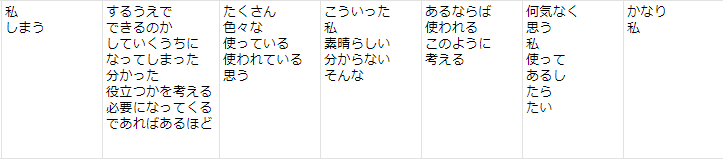
\includegraphics[width=150mm]{image/kenshutukekka-a.png}
	\label{kenshutukekka}
\end{table}
\begin{table}[H]
    \centering
    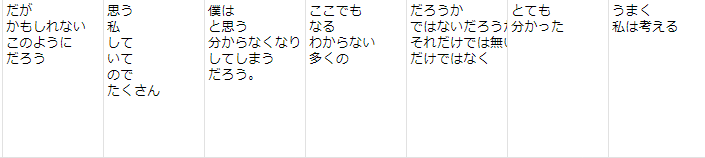
\includegraphics[width=150mm]{image/kenshutukekka-b.png}
    \label{kenshutukekka-2}
\end{table}

書きことばリストにあげている表現を検出した個数は60個である.書きことばリストに含まれている表現の個数をまとめた表を表\ref{kenshutu-ichiran-old}に示す.

\begin{table}[H]
	\centering
        \caption{話しことばチェッカーの話しことば検出画面}
 	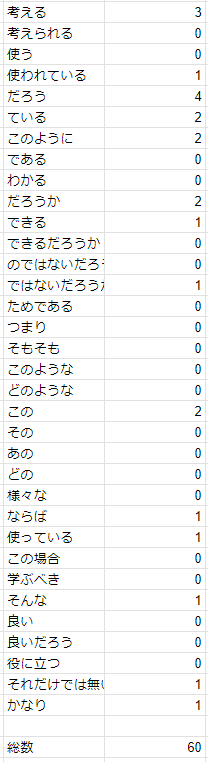
\includegraphics[width=55mm]{image/kenshutu-ichiran-old.png}
	\label{kenshutu-ichiran-old}
\end{table}

\section{書きことばリストを用いた検証 \label{c7s2}}
書きことばリストをプロンプトに組み込み,誤検出の減少を図ったが,明らかな減少は見られなかった.書きことばリストにあげられている表現が依然として多く,得られた出力結果をを用いて,書きことばリストに載っている表現を除去するように再度指示を与えた.

\begin{table}[H]
\centering
\caption{話しことば検出のためのプロンプト(後半部)}
\small % \footnotesize
\begin{tabular}{|l|}
\hline
\multicolumn{1}{|c|}{プロンプト} \\ \hline
\begin{tabular}[c]{@{}l@{}} 
\#\#\# 指示 \#\#\# \\
以下の<書きことばリスト>の1から34までの表現は書きことばとします。<書きことばリスト>の言葉が\#\#\# 表現リスト \#\#\#に含まれている場合、\#\#\# 表現リスト \#\#\#から除外して出力してください。
<書きことばリスト>
1. 考える
2. 考えられる
3. 使う
4. 使われている
5. だろう
6. ている
7. このように
8. である
9. わかる
10. だろうか
11. できる
12. できるだろうか
13. のではないだろうか
14. ではないだろうか
15. ためである
16. つまり
17. そもそも
18. このような
19. どのような
20. この
21. その
22. あの
23. どの
24. 様々な
25. ならば
26. 使っている
27. この場合
28. 学ぶべき
29. そんな
30. 良い
31. 良いだろう
32. 役に立つ
33. それだけでは無い
34. かなり

\#\#\# 表現リスト \#\#\# \\
(1度目の出力で得られた「話しことばとされたもの」)
\end{tabular}   \\ \hline

\end{tabular}
\label{prompt-sdetectspoken-klist}
\end{table} % なぜこのプロンプトにしたか書こう


プロンプトの内容は,表\ref{prompt-detectspoken-api},表\ref{prompt-sdetectspoken-klist}の書きことばリストの部分を抜き取り,\ref{c7s1}節の結果から書きことばリストに当てはまる表現を除去する内容である.

\subsection{結果}
上記のプロンプトで得られた話しことば検出結果を表\ref{kenshutu-ichiran-imp}に示す.

\begin{table}[H]
	\centering
        \caption{話しことばチェッカーの話しことば検出画面}
 	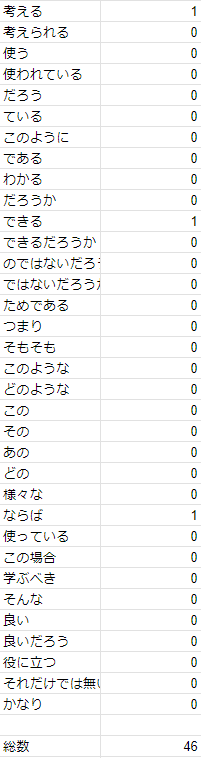
\includegraphics[width=55mm]{image/kenshutu-ichiran-imp.png}
	\label{kenshutu-ichiran-imp}
\end{table}

\subsection{考察}
指示を二段階に分けることにより,明らかな書きことばの減少が確認できた.一度の処理では,ChatGPTは最初に書かれた指示を優先して行い,その後の指示を読み取ることが難しいと考えられる.

\section{話しことばの具体例を用いた検証}
\section{}
\begin{comment}
    1. checkerの基本性能
    2. プロンプトによる話しことば検出
    3. データ整理
        Few-shot: 例文と話しことば
        Few-shot+書きことばリスト
        Few-shot+話しことば例+書きことばリスト
        プロンプト調整
    4. 改良プロンプトによる話しことば検出

    第5章追記準備
    第7章用整理
\end{comment}

\begin{comment}
    本章では,話しことば検出におけるLLMの性能調査を行い,
    LLMの話しことばの理解と,データ収集における利用可能性について模索する.

    構成...?
    実験内容→プロンプト→結果→考察

    
\end{comment}

\begin{comment}
本実験で用いたデータは,本学で2019年度に開講された「アルゴリズムとプログラミング」の講義内で課されたレポートから16件のレポート本文である.本章で述べる検証では一律でこのデータを使用した.
    (1. GPT-4による話しことば検出)
    プロンプトに,話しことばを検出
    2. 短文とその時の話しことば検出結果の組を1つの例とし,プロンプトの例示の部分に組み込んだものを使用し話しことば検出を行った.この時に使用した短文は,話しことば事例集から抜粋したものである.
    3. 明らかに書きことばとされる表現を挿入した
    4. 2に例示の形式を変更し加えたものを与えた
    5. 上記の結果を踏まえ,プロンプトの文言を編集した
    6. 専門家による判定
\end{comment}